% Created by tikzDevice version 0.12.6 on 2025-10-13 00:35:54
% !TEX encoding = UTF-8 Unicode
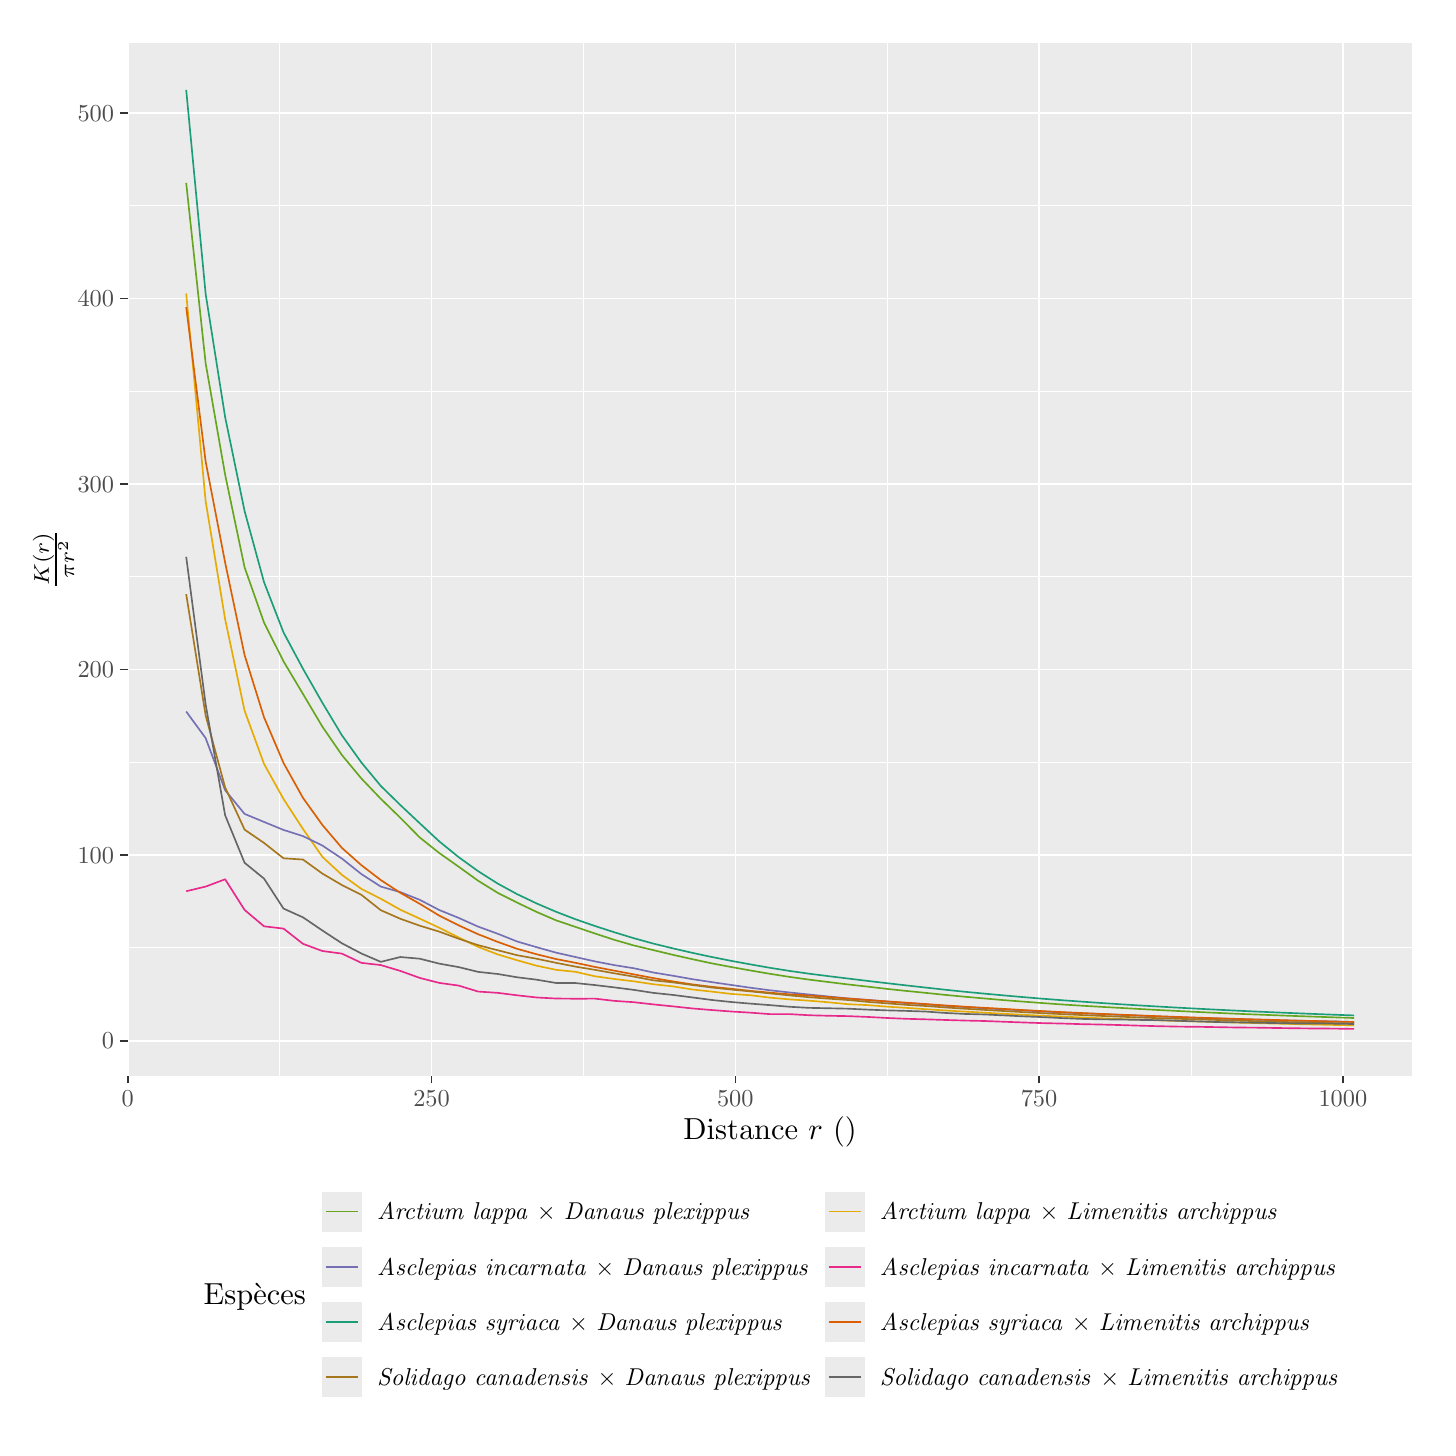
\begin{tikzpicture}[x=1pt,y=1pt]
\definecolor{fillColor}{RGB}{255,255,255}
\path[use as bounding box,fill=fillColor,fill opacity=0.00] (0,0) rectangle (505.89,505.89);
\begin{scope}
\path[clip] (  0.00,  0.00) rectangle (505.89,505.89);
\definecolor{drawColor}{RGB}{255,255,255}
\definecolor{fillColor}{RGB}{255,255,255}

\path[draw=drawColor,line width= 0.6pt,line join=round,line cap=round,fill=fillColor] (  0.00,  0.00) rectangle (505.89,505.89);
\end{scope}
\begin{scope}
\path[clip] ( 36.18,127.12) rectangle (500.39,500.39);
\definecolor{fillColor}{gray}{0.92}

\path[fill=fillColor] ( 36.18,127.12) rectangle (500.39,500.39);
\definecolor{drawColor}{RGB}{255,255,255}

\path[draw=drawColor,line width= 0.3pt,line join=round] ( 36.18,173.36) --
	(500.39,173.36);

\path[draw=drawColor,line width= 0.3pt,line join=round] ( 36.18,240.41) --
	(500.39,240.41);

\path[draw=drawColor,line width= 0.3pt,line join=round] ( 36.18,307.46) --
	(500.39,307.46);

\path[draw=drawColor,line width= 0.3pt,line join=round] ( 36.18,374.50) --
	(500.39,374.50);

\path[draw=drawColor,line width= 0.3pt,line join=round] ( 36.18,441.55) --
	(500.39,441.55);

\path[draw=drawColor,line width= 0.3pt,line join=round] ( 91.06,127.12) --
	( 91.06,500.39);

\path[draw=drawColor,line width= 0.3pt,line join=round] (200.83,127.12) --
	(200.83,500.39);

\path[draw=drawColor,line width= 0.3pt,line join=round] (310.59,127.12) --
	(310.59,500.39);

\path[draw=drawColor,line width= 0.3pt,line join=round] (420.35,127.12) --
	(420.35,500.39);

\path[draw=drawColor,line width= 0.6pt,line join=round] ( 36.18,139.84) --
	(500.39,139.84);

\path[draw=drawColor,line width= 0.6pt,line join=round] ( 36.18,206.89) --
	(500.39,206.89);

\path[draw=drawColor,line width= 0.6pt,line join=round] ( 36.18,273.93) --
	(500.39,273.93);

\path[draw=drawColor,line width= 0.6pt,line join=round] ( 36.18,340.98) --
	(500.39,340.98);

\path[draw=drawColor,line width= 0.6pt,line join=round] ( 36.18,408.03) --
	(500.39,408.03);

\path[draw=drawColor,line width= 0.6pt,line join=round] ( 36.18,475.07) --
	(500.39,475.07);

\path[draw=drawColor,line width= 0.6pt,line join=round] ( 36.18,127.12) --
	( 36.18,500.39);

\path[draw=drawColor,line width= 0.6pt,line join=round] (145.94,127.12) --
	(145.94,500.39);

\path[draw=drawColor,line width= 0.6pt,line join=round] (255.71,127.12) --
	(255.71,500.39);

\path[draw=drawColor,line width= 0.6pt,line join=round] (365.47,127.12) --
	(365.47,500.39);

\path[draw=drawColor,line width= 0.6pt,line join=round] (475.24,127.12) --
	(475.24,500.39);
\definecolor{drawColor}{RGB}{102,166,30}

\path[draw=drawColor,line width= 0.6pt,line join=round] ( 57.28,449.77) --
	( 64.31,384.61) --
	( 71.35,344.36) --
	( 78.38,310.88) --
	( 85.41,290.90) --
	( 92.45,276.91) --
	( 99.48,265.12) --
	(106.51,253.28) --
	(113.55,243.05) --
	(120.58,234.58) --
	(127.61,227.23) --
	(134.65,220.39) --
	(141.68,213.26) --
	(148.72,207.65) --
	(155.75,202.69) --
	(162.78,197.62) --
	(169.82,193.28) --
	(176.85,189.73) --
	(183.88,186.37) --
	(190.92,183.33) --
	(197.95,180.95) --
	(204.98,178.57) --
	(212.02,176.26) --
	(219.05,174.24) --
	(226.08,172.56) --
	(233.12,170.87) --
	(240.15,169.29) --
	(247.18,167.78) --
	(254.22,166.45) --
	(261.25,165.19) --
	(268.28,163.99) --
	(275.32,162.88) --
	(282.35,161.90) --
	(289.39,161.02) --
	(296.42,160.16) --
	(303.45,159.37) --
	(310.49,158.55) --
	(317.52,157.81) --
	(324.55,157.11) --
	(331.59,156.38) --
	(338.62,155.72) --
	(345.65,155.10) --
	(352.69,154.49) --
	(359.72,153.95) --
	(366.75,153.43) --
	(373.79,152.92) --
	(380.82,152.48) --
	(387.85,152.07) --
	(394.89,151.68) --
	(401.92,151.28) --
	(408.95,150.90) --
	(415.99,150.55) --
	(423.02,150.20) --
	(430.06,149.87) --
	(437.09,149.56) --
	(444.12,149.28) --
	(451.16,149.01) --
	(458.19,148.75) --
	(465.22,148.51) --
	(472.26,148.26) --
	(479.29,148.03);
\definecolor{drawColor}{RGB}{230,171,2}

\path[draw=drawColor,line width= 0.6pt,line join=round] ( 57.28,409.82) --
	( 64.31,334.73) --
	( 71.35,292.11) --
	( 78.38,259.08) --
	( 85.41,239.84) --
	( 92.45,227.16) --
	( 99.48,216.33) --
	(106.51,206.25) --
	(113.55,199.75) --
	(120.58,194.68) --
	(127.61,191.12) --
	(134.65,187.16) --
	(141.68,183.94) --
	(148.72,180.65) --
	(155.75,177.11) --
	(162.78,173.71) --
	(169.82,171.03) --
	(176.85,168.90) --
	(183.88,166.93) --
	(190.92,165.44) --
	(197.95,164.72) --
	(204.98,163.11) --
	(212.02,162.13) --
	(219.05,161.29) --
	(226.08,160.23) --
	(233.12,159.47) --
	(240.15,158.33) --
	(247.18,157.57) --
	(254.22,156.74) --
	(261.25,156.25) --
	(268.28,155.38) --
	(275.32,154.76) --
	(282.35,154.29) --
	(289.39,153.71) --
	(296.42,153.03) --
	(303.45,152.69) --
	(310.49,152.14) --
	(317.52,151.69) --
	(324.55,151.21) --
	(331.59,150.75) --
	(338.62,150.35) --
	(345.65,149.96) --
	(352.69,149.56) --
	(359.72,149.18) --
	(366.75,148.84) --
	(373.79,148.56) --
	(380.82,148.22) --
	(387.85,147.94) --
	(394.89,147.66) --
	(401.92,147.43) --
	(408.95,147.18) --
	(415.99,146.95) --
	(423.02,146.78) --
	(430.06,146.56) --
	(437.09,146.37) --
	(444.12,146.18) --
	(451.16,146.01) --
	(458.19,145.83) --
	(465.22,145.68) --
	(472.26,145.52) --
	(479.29,145.38);
\definecolor{drawColor}{RGB}{117,112,179}

\path[draw=drawColor,line width= 0.6pt,line join=round] ( 57.28,258.78) --
	( 64.31,249.17) --
	( 71.35,230.35) --
	( 78.38,221.79) --
	( 85.41,218.88) --
	( 92.45,215.99) --
	( 99.48,213.76) --
	(106.51,210.34) --
	(113.55,205.65) --
	(120.58,200.04) --
	(127.61,195.51) --
	(134.65,193.52) --
	(141.68,190.74) --
	(148.72,187.06) --
	(155.75,184.20) --
	(162.78,181.05) --
	(169.82,178.49) --
	(176.85,175.68) --
	(183.88,173.63) --
	(190.92,171.65) --
	(197.95,170.06) --
	(204.98,168.49) --
	(212.02,167.13) --
	(219.05,166.01) --
	(226.08,164.47) --
	(233.12,163.31) --
	(240.15,162.07) --
	(247.18,161.00) --
	(254.22,159.97) --
	(261.25,158.96) --
	(268.28,158.04) --
	(275.32,157.26) --
	(282.35,156.52) --
	(289.39,155.80) --
	(296.42,155.10) --
	(303.45,154.58) --
	(310.49,154.00) --
	(317.52,153.41) --
	(324.55,152.94) --
	(331.59,152.42) --
	(338.62,151.99) --
	(345.65,151.54) --
	(352.69,151.15) --
	(359.72,150.76) --
	(366.75,150.39) --
	(373.79,150.04) --
	(380.82,149.73) --
	(387.85,149.47) --
	(394.89,149.16) --
	(401.92,148.88) --
	(408.95,148.57) --
	(415.99,148.32) --
	(423.02,148.06) --
	(430.06,147.87) --
	(437.09,147.64) --
	(444.12,147.43) --
	(451.16,147.22) --
	(458.19,147.05) --
	(465.22,146.94) --
	(472.26,146.78) --
	(479.29,146.60);
\definecolor{drawColor}{RGB}{231,41,138}

\path[draw=drawColor,line width= 0.6pt,line join=round] ( 57.28,193.84) --
	( 64.31,195.52) --
	( 71.35,198.16) --
	( 78.38,187.09) --
	( 85.41,181.16) --
	( 92.45,180.34) --
	( 99.48,174.84) --
	(106.51,172.24) --
	(113.55,171.30) --
	(120.58,167.96) --
	(127.61,167.16) --
	(134.65,165.05) --
	(141.68,162.52) --
	(148.72,160.72) --
	(155.75,159.74) --
	(162.78,157.59) --
	(169.82,157.12) --
	(176.85,156.24) --
	(183.88,155.45) --
	(190.92,155.07) --
	(197.95,155.00) --
	(204.98,155.03) --
	(212.02,154.22) --
	(219.05,153.74) --
	(226.08,152.95) --
	(233.12,152.24) --
	(240.15,151.49) --
	(247.18,150.91) --
	(254.22,150.38) --
	(261.25,149.96) --
	(268.28,149.43) --
	(275.32,149.44) --
	(282.35,149.03) --
	(289.39,148.84) --
	(296.42,148.71) --
	(303.45,148.42) --
	(310.49,148.04) --
	(317.52,147.74) --
	(324.55,147.55) --
	(331.59,147.32) --
	(338.62,147.11) --
	(345.65,146.95) --
	(352.69,146.68) --
	(359.72,146.42) --
	(366.75,146.18) --
	(373.79,146.03) --
	(380.82,145.81) --
	(387.85,145.67) --
	(394.89,145.48) --
	(401.92,145.26) --
	(408.95,145.06) --
	(415.99,144.92) --
	(423.02,144.85) --
	(430.06,144.72) --
	(437.09,144.60) --
	(444.12,144.54) --
	(451.16,144.42) --
	(458.19,144.32) --
	(465.22,144.24) --
	(472.26,144.20) --
	(479.29,144.09);
\definecolor{drawColor}{RGB}{27,158,119}

\path[draw=drawColor,line width= 0.6pt,line join=round] ( 57.28,483.42) --
	( 64.31,409.69) --
	( 71.35,365.19) --
	( 78.38,331.22) --
	( 85.41,305.51) --
	( 92.45,287.35) --
	( 99.48,274.23) --
	(106.51,261.91) --
	(113.55,250.18) --
	(120.58,240.37) --
	(127.61,231.88) --
	(134.65,225.00) --
	(141.68,218.39) --
	(148.72,211.86) --
	(155.75,206.14) --
	(162.78,201.08) --
	(169.82,196.62) --
	(176.85,192.79) --
	(183.88,189.44) --
	(190.92,186.42) --
	(197.95,183.72) --
	(204.98,181.27) --
	(212.02,179.00) --
	(219.05,176.86) --
	(226.08,174.92) --
	(233.12,173.20) --
	(240.15,171.58) --
	(247.18,170.08) --
	(254.22,168.68) --
	(261.25,167.39) --
	(268.28,166.16) --
	(275.32,165.04) --
	(282.35,164.05) --
	(289.39,163.15) --
	(296.42,162.30) --
	(303.45,161.44) --
	(310.49,160.61) --
	(317.52,159.81) --
	(324.55,159.02) --
	(331.59,158.24) --
	(338.62,157.51) --
	(345.65,156.84) --
	(352.69,156.20) --
	(359.72,155.58) --
	(366.75,155.00) --
	(373.79,154.46) --
	(380.82,153.95) --
	(387.85,153.46) --
	(394.89,153.00) --
	(401.92,152.56) --
	(408.95,152.15) --
	(415.99,151.75) --
	(423.02,151.38) --
	(430.06,151.02) --
	(437.09,150.68) --
	(444.12,150.35) --
	(451.16,150.05) --
	(458.19,149.76) --
	(465.22,149.48) --
	(472.26,149.21) --
	(479.29,148.96);
\definecolor{drawColor}{RGB}{217,95,2}

\path[draw=drawColor,line width= 0.6pt,line join=round] ( 57.28,404.92) --
	( 64.31,349.10) --
	( 71.35,312.60) --
	( 78.38,279.17) --
	( 85.41,256.68) --
	( 92.45,240.19) --
	( 99.48,227.57) --
	(106.51,217.76) --
	(113.55,209.49) --
	(120.58,203.26) --
	(127.61,197.87) --
	(134.65,193.27) --
	(141.68,189.30) --
	(148.72,185.03) --
	(155.75,181.50) --
	(162.78,178.30) --
	(169.82,175.54) --
	(176.85,173.04) --
	(183.88,171.07) --
	(190.92,169.34) --
	(197.95,167.98) --
	(204.98,166.48) --
	(212.02,165.13) --
	(219.05,163.79) --
	(226.08,162.45) --
	(233.12,161.26) --
	(240.15,160.18) --
	(247.18,159.30) --
	(254.22,158.59) --
	(261.25,157.83) --
	(268.28,157.18) --
	(275.32,156.58) --
	(282.35,156.16) --
	(289.39,155.60) --
	(296.42,155.06) --
	(303.45,154.53) --
	(310.49,154.02) --
	(317.52,153.57) --
	(324.55,153.08) --
	(331.59,152.56) --
	(338.62,152.11) --
	(345.65,151.71) --
	(352.69,151.32) --
	(359.72,150.90) --
	(366.75,150.52) --
	(373.79,150.15) --
	(380.82,149.83) --
	(387.85,149.51) --
	(394.89,149.22) --
	(401.92,148.94) --
	(408.95,148.66) --
	(415.99,148.40) --
	(423.02,148.15) --
	(430.06,147.92) --
	(437.09,147.70) --
	(444.12,147.50) --
	(451.16,147.31) --
	(458.19,147.11) --
	(465.22,146.93) --
	(472.26,146.76) --
	(479.29,146.59);
\definecolor{drawColor}{RGB}{166,118,29}

\path[draw=drawColor,line width= 0.6pt,line join=round] ( 57.28,301.19) --
	( 64.31,257.33) --
	( 71.35,231.35) --
	( 78.38,216.10) --
	( 85.41,211.29) --
	( 92.45,205.74) --
	( 99.48,205.29) --
	(106.51,200.21) --
	(113.55,196.07) --
	(120.58,192.54) --
	(127.61,186.98) --
	(134.65,183.89) --
	(141.68,181.39) --
	(148.72,179.24) --
	(155.75,176.67) --
	(162.78,174.35) --
	(169.82,172.52) --
	(176.85,170.72) --
	(183.88,169.45) --
	(190.92,167.97) --
	(197.95,166.60) --
	(204.98,165.43) --
	(212.02,164.17) --
	(219.05,162.98) --
	(226.08,161.64) --
	(233.12,160.90) --
	(240.15,159.95) --
	(247.18,159.05) --
	(254.22,158.30) --
	(261.25,157.64) --
	(268.28,156.91) --
	(275.32,156.20) --
	(282.35,155.54) --
	(289.39,155.02) --
	(296.42,154.53) --
	(303.45,153.86) --
	(310.49,153.32) --
	(317.52,152.78) --
	(324.55,152.36) --
	(331.59,151.84) --
	(338.62,151.38) --
	(345.65,150.96) --
	(352.69,150.55) --
	(359.72,150.15) --
	(366.75,149.77) --
	(373.79,149.43) --
	(380.82,149.10) --
	(387.85,148.79) --
	(394.89,148.50) --
	(401.92,148.21) --
	(408.95,147.96) --
	(415.99,147.73) --
	(423.02,147.54) --
	(430.06,147.31) --
	(437.09,147.10) --
	(444.12,146.88) --
	(451.16,146.67) --
	(458.19,146.49) --
	(465.22,146.35) --
	(472.26,146.18) --
	(479.29,146.05);
\definecolor{drawColor}{gray}{0.40}

\path[draw=drawColor,line width= 0.6pt,line join=round] ( 57.28,314.68) --
	( 64.31,261.33) --
	( 71.35,221.30) --
	( 78.38,204.12) --
	( 85.41,198.40) --
	( 92.45,187.57) --
	( 99.48,184.41) --
	(106.51,179.64) --
	(113.55,175.03) --
	(120.58,171.34) --
	(127.61,168.32) --
	(134.65,170.07) --
	(141.68,169.46) --
	(148.72,167.68) --
	(155.75,166.42) --
	(162.78,164.70) --
	(169.82,163.94) --
	(176.85,162.75) --
	(183.88,161.88) --
	(190.92,160.69) --
	(197.95,160.66) --
	(204.98,159.93) --
	(212.02,159.09) --
	(219.05,158.19) --
	(226.08,157.11) --
	(233.12,156.37) --
	(240.15,155.47) --
	(247.18,154.55) --
	(254.22,153.81) --
	(261.25,153.22) --
	(268.28,152.68) --
	(275.32,152.09) --
	(282.35,151.70) --
	(289.39,151.55) --
	(296.42,151.40) --
	(303.45,151.06) --
	(310.49,150.79) --
	(317.52,150.60) --
	(324.55,150.36) --
	(331.59,149.86) --
	(338.62,149.50) --
	(345.65,149.31) --
	(352.69,148.98) --
	(359.72,148.63) --
	(366.75,148.35) --
	(373.79,148.00) --
	(380.82,147.71) --
	(387.85,147.54) --
	(394.89,147.49) --
	(401.92,147.34) --
	(408.95,147.25) --
	(415.99,147.01) --
	(423.02,146.79) --
	(430.06,146.57) --
	(437.09,146.45) --
	(444.12,146.31) --
	(451.16,146.20) --
	(458.19,146.06) --
	(465.22,146.06) --
	(472.26,145.98) --
	(479.29,145.86);
\end{scope}
\begin{scope}
\path[clip] (  0.00,  0.00) rectangle (505.89,505.89);
\definecolor{drawColor}{gray}{0.30}

\node[text=drawColor,anchor=base east,inner sep=0pt, outer sep=0pt, scale=  0.88] at ( 31.23,136.84) {0};

\node[text=drawColor,anchor=base east,inner sep=0pt, outer sep=0pt, scale=  0.88] at ( 31.23,203.88) {100};

\node[text=drawColor,anchor=base east,inner sep=0pt, outer sep=0pt, scale=  0.88] at ( 31.23,270.93) {200};

\node[text=drawColor,anchor=base east,inner sep=0pt, outer sep=0pt, scale=  0.88] at ( 31.23,337.97) {300};

\node[text=drawColor,anchor=base east,inner sep=0pt, outer sep=0pt, scale=  0.88] at ( 31.23,405.02) {400};

\node[text=drawColor,anchor=base east,inner sep=0pt, outer sep=0pt, scale=  0.88] at ( 31.23,472.07) {500};
\end{scope}
\begin{scope}
\path[clip] (  0.00,  0.00) rectangle (505.89,505.89);
\definecolor{drawColor}{gray}{0.20}

\path[draw=drawColor,line width= 0.6pt,line join=round] ( 33.43,139.84) --
	( 36.18,139.84);

\path[draw=drawColor,line width= 0.6pt,line join=round] ( 33.43,206.89) --
	( 36.18,206.89);

\path[draw=drawColor,line width= 0.6pt,line join=round] ( 33.43,273.93) --
	( 36.18,273.93);

\path[draw=drawColor,line width= 0.6pt,line join=round] ( 33.43,340.98) --
	( 36.18,340.98);

\path[draw=drawColor,line width= 0.6pt,line join=round] ( 33.43,408.03) --
	( 36.18,408.03);

\path[draw=drawColor,line width= 0.6pt,line join=round] ( 33.43,475.07) --
	( 36.18,475.07);
\end{scope}
\begin{scope}
\path[clip] (  0.00,  0.00) rectangle (505.89,505.89);
\definecolor{drawColor}{gray}{0.20}

\path[draw=drawColor,line width= 0.6pt,line join=round] ( 36.18,124.37) --
	( 36.18,127.12);

\path[draw=drawColor,line width= 0.6pt,line join=round] (145.94,124.37) --
	(145.94,127.12);

\path[draw=drawColor,line width= 0.6pt,line join=round] (255.71,124.37) --
	(255.71,127.12);

\path[draw=drawColor,line width= 0.6pt,line join=round] (365.47,124.37) --
	(365.47,127.12);

\path[draw=drawColor,line width= 0.6pt,line join=round] (475.24,124.37) --
	(475.24,127.12);
\end{scope}
\begin{scope}
\path[clip] (  0.00,  0.00) rectangle (505.89,505.89);
\definecolor{drawColor}{gray}{0.30}

\node[text=drawColor,anchor=base,inner sep=0pt, outer sep=0pt, scale=  0.88] at ( 36.18,116.16) {0};

\node[text=drawColor,anchor=base,inner sep=0pt, outer sep=0pt, scale=  0.88] at (145.94,116.16) {250};

\node[text=drawColor,anchor=base,inner sep=0pt, outer sep=0pt, scale=  0.88] at (255.71,116.16) {500};

\node[text=drawColor,anchor=base,inner sep=0pt, outer sep=0pt, scale=  0.88] at (365.47,116.16) {750};

\node[text=drawColor,anchor=base,inner sep=0pt, outer sep=0pt, scale=  0.88] at (475.24,116.16) {1000};
\end{scope}
\begin{scope}
\path[clip] (  0.00,  0.00) rectangle (505.89,505.89);
\definecolor{drawColor}{RGB}{0,0,0}

\node[text=drawColor,anchor=base,inner sep=0pt, outer sep=0pt, scale=  1.10] at (268.28,104.08) {Distance $r$ (\unit{\m})};
\end{scope}
\begin{scope}
\path[clip] (  0.00,  0.00) rectangle (505.89,505.89);
\definecolor{drawColor}{RGB}{0,0,0}

\node[text=drawColor,rotate= 90.00,anchor=base,inner sep=0pt, outer sep=0pt, scale=  1.10] at ( 13.01,313.75) {$\frac{K(r)}{\pi r^2}$};
\end{scope}
\begin{scope}
\path[clip] (  0.00,  0.00) rectangle (505.89,505.89);
\definecolor{fillColor}{RGB}{255,255,255}

\path[fill=fillColor] ( 58.08,  5.50) rectangle (478.49, 90.82);
\end{scope}
\begin{scope}
\path[clip] (  0.00,  0.00) rectangle (505.89,505.89);
\definecolor{drawColor}{RGB}{0,0,0}

\node[text=drawColor,anchor=base west,inner sep=0pt, outer sep=0pt, scale=  1.10] at ( 63.58, 44.40) {Espèces};
\end{scope}
\begin{scope}
\path[clip] (  0.00,  0.00) rectangle (505.89,505.89);
\definecolor{fillColor}{gray}{0.92}

\path[fill=fillColor] (106.31, 70.86) rectangle (120.77, 85.32);
\definecolor{drawColor}{RGB}{102,166,30}

\path[draw=drawColor,line width= 0.6pt,line join=round] (107.76, 78.09) -- (119.32, 78.09);
\end{scope}
\begin{scope}
\path[clip] (  0.00,  0.00) rectangle (505.89,505.89);
\definecolor{fillColor}{gray}{0.92}

\path[fill=fillColor] (287.98, 70.86) rectangle (302.43, 85.32);
\definecolor{drawColor}{RGB}{230,171,2}

\path[draw=drawColor,line width= 0.6pt,line join=round] (289.42, 78.09) -- (300.98, 78.09);
\end{scope}
\begin{scope}
\path[clip] (  0.00,  0.00) rectangle (505.89,505.89);
\definecolor{fillColor}{gray}{0.92}

\path[fill=fillColor] (106.31, 50.91) rectangle (120.77, 65.36);
\definecolor{drawColor}{RGB}{117,112,179}

\path[draw=drawColor,line width= 0.6pt,line join=round] (107.76, 58.14) -- (119.32, 58.14);
\end{scope}
\begin{scope}
\path[clip] (  0.00,  0.00) rectangle (505.89,505.89);
\definecolor{fillColor}{gray}{0.92}

\path[fill=fillColor] (287.98, 50.91) rectangle (302.43, 65.36);
\definecolor{drawColor}{RGB}{231,41,138}

\path[draw=drawColor,line width= 0.6pt,line join=round] (289.42, 58.14) -- (300.98, 58.14);
\end{scope}
\begin{scope}
\path[clip] (  0.00,  0.00) rectangle (505.89,505.89);
\definecolor{fillColor}{gray}{0.92}

\path[fill=fillColor] (106.31, 30.95) rectangle (120.77, 45.41);
\definecolor{drawColor}{RGB}{27,158,119}

\path[draw=drawColor,line width= 0.6pt,line join=round] (107.76, 38.18) -- (119.32, 38.18);
\end{scope}
\begin{scope}
\path[clip] (  0.00,  0.00) rectangle (505.89,505.89);
\definecolor{fillColor}{gray}{0.92}

\path[fill=fillColor] (287.98, 30.95) rectangle (302.43, 45.41);
\definecolor{drawColor}{RGB}{217,95,2}

\path[draw=drawColor,line width= 0.6pt,line join=round] (289.42, 38.18) -- (300.98, 38.18);
\end{scope}
\begin{scope}
\path[clip] (  0.00,  0.00) rectangle (505.89,505.89);
\definecolor{fillColor}{gray}{0.92}

\path[fill=fillColor] (106.31, 11.00) rectangle (120.77, 25.45);
\definecolor{drawColor}{RGB}{166,118,29}

\path[draw=drawColor,line width= 0.6pt,line join=round] (107.76, 18.23) -- (119.32, 18.23);
\end{scope}
\begin{scope}
\path[clip] (  0.00,  0.00) rectangle (505.89,505.89);
\definecolor{fillColor}{gray}{0.92}

\path[fill=fillColor] (287.98, 11.00) rectangle (302.43, 25.45);
\definecolor{drawColor}{gray}{0.40}

\path[draw=drawColor,line width= 0.6pt,line join=round] (289.42, 18.23) -- (300.98, 18.23);
\end{scope}
\begin{scope}
\path[clip] (  0.00,  0.00) rectangle (505.89,505.89);
\definecolor{drawColor}{RGB}{0,0,0}

\node[text=drawColor,anchor=base west,inner sep=0pt, outer sep=0pt, scale=  0.88] at (126.27, 75.08) {\textit{Arctium lappa} $\times$ \textit{Danaus plexippus}};
\end{scope}
\begin{scope}
\path[clip] (  0.00,  0.00) rectangle (505.89,505.89);
\definecolor{drawColor}{RGB}{0,0,0}

\node[text=drawColor,anchor=base west,inner sep=0pt, outer sep=0pt, scale=  0.88] at (307.93, 75.08) {\textit{Arctium lappa} $\times$ \textit{Limenitis archippus}};
\end{scope}
\begin{scope}
\path[clip] (  0.00,  0.00) rectangle (505.89,505.89);
\definecolor{drawColor}{RGB}{0,0,0}

\node[text=drawColor,anchor=base west,inner sep=0pt, outer sep=0pt, scale=  0.88] at (126.27, 55.13) {\textit{Asclepias incarnata} $\times$ \textit{Danaus plexippus}};
\end{scope}
\begin{scope}
\path[clip] (  0.00,  0.00) rectangle (505.89,505.89);
\definecolor{drawColor}{RGB}{0,0,0}

\node[text=drawColor,anchor=base west,inner sep=0pt, outer sep=0pt, scale=  0.88] at (307.93, 55.13) {\textit{Asclepias incarnata} $\times$ \textit{Limenitis archippus}};
\end{scope}
\begin{scope}
\path[clip] (  0.00,  0.00) rectangle (505.89,505.89);
\definecolor{drawColor}{RGB}{0,0,0}

\node[text=drawColor,anchor=base west,inner sep=0pt, outer sep=0pt, scale=  0.88] at (126.27, 35.18) {\textit{Asclepias syriaca} $\times$ \textit{Danaus plexippus}};
\end{scope}
\begin{scope}
\path[clip] (  0.00,  0.00) rectangle (505.89,505.89);
\definecolor{drawColor}{RGB}{0,0,0}

\node[text=drawColor,anchor=base west,inner sep=0pt, outer sep=0pt, scale=  0.88] at (307.93, 35.18) {\textit{Asclepias syriaca} $\times$ \textit{Limenitis archippus}};
\end{scope}
\begin{scope}
\path[clip] (  0.00,  0.00) rectangle (505.89,505.89);
\definecolor{drawColor}{RGB}{0,0,0}

\node[text=drawColor,anchor=base west,inner sep=0pt, outer sep=0pt, scale=  0.88] at (126.27, 15.22) {\textit{Solidago canadensis} $\times$ \textit{Danaus plexippus}};
\end{scope}
\begin{scope}
\path[clip] (  0.00,  0.00) rectangle (505.89,505.89);
\definecolor{drawColor}{RGB}{0,0,0}

\node[text=drawColor,anchor=base west,inner sep=0pt, outer sep=0pt, scale=  0.88] at (307.93, 15.22) {\textit{Solidago canadensis} $\times$ \textit{Limenitis archippus}};
\end{scope}
\end{tikzpicture}
